\documentclass[ignorenonframetext,plain,fleqn]{beamer}
\setbeamertemplate{navigation symbols}{}

\newcommand{\vocab}{\mathcal{V}}
\newcommand{\corpus}{\mathcal{C}}
\newcommand{\pml}{p_{\textsc{ml}}}
\DeclareMathOperator*{\argmax}{argmax}
\DeclareMathOperator*{\argmin}{argmin}
\newcommand{\score}{\mathit{score}}
\newcommand{\loss}{\mathit{loss}}
\renewcommand{\vec}{\mathbf}
\newcommand{\pluseq}{\mathrel{+}=}

\title{Learning to map strings to classes}
\subtitle{Comp 542 Natural Language Processing}
\author{Deniz Yuret}

\hypersetup{colorlinks,urlcolor=red}

\begin{document}

\begin{frame}
\maketitle
\end{frame}

\begin{frame}\frametitle{Applications}
\begin{itemize}
\item
  \href{http://en.wikipedia.org/wiki/Document_classification}{Document
    classification}: Text $\rightarrow$ \{ politics, finance, $\dots$ \}
\begin{itemize}
\item See \href{http://www-nlp.stanford.edu/IR-book}{Introduction to
  Information Retrieval} Chapter 13,
  \href{http://nlp.stanford.edu/fsnlp}{Foundations of Statistical NLP}
  Chapter 16 for an introduction.
\item Some datasets: \href{http://qwone.com/~jason/20Newsgroups}{20 Newsgroups},
  \href{http://www.daviddlewis.com/resources/testcollections/reuters21578}{Reuters
    21578}, 
  \href{http://www.ai.mit.edu/projects/jmlr/papers/volume5/lewis04a/lyrl2004_rcv1v2_README.htm}{Reuters
    RCV1}, and \href{http://www.cs.cmu.edu/~webkb/}{WebKB}.
\item More datasets available at \href{http://kdd.ics.uci.edu}{UCI
  KDD}, \href{http://archive.ics.uci.edu/ml/index.html}{ML},
  \href{http://csmining.org/index.php/data.html}{CSMining},
  \href{http://www.cs.cmu.edu/~TextLearning/datasets.html}{CMU}.
\end{itemize}
\item \href{http://en.wikipedia.org/wiki/Sentiment_analysis}{Sentiment
  analysis}: Text $\rightarrow$ \{ positive, negative \}
\begin{itemize}
\item
  \href{http://www.cs.cornell.edu/home/llee/opinion-mining-sentiment-analysis-survey.html}{Survey
    book} by Pang and Lee.
\item
  \href{http://www.cs.cornell.edu/people/pabo/movie-review-data}{Movie
    review data} by Pang and Lee.
\end{itemize}
\item \href{http://en.wikipedia.org/wiki/Anti-spam_techniques}{Spam
  detection}: Text $\rightarrow$ \{ spam, regular \}
\begin{itemize}
\item
  \href{http://www.aclweb.org/aclwiki/index.php?title=Spam_filtering_datasets}{Spam
  filtering datasets} from ACL Wiki.
\item \href{http://csmining.org/index.php/data.html}{Other datasets} from
  CSMining Group.
\item \href{http://archive.ics.uci.edu/ml/datasets/Spambase}{Spambase}
  from UCI machine learning repository.
\end{itemize}
\end{itemize}
\end{frame}

\begin{frame}\frametitle{String classification models}
We need to learn a function for classification from examples:\[
f: \mathcal{X}\rightarrow\mathcal{Y}
\] where $x\in\mathcal{X}$ is a string and
$\mathcal{Y}$ is a small list of classes.  This is typically done
by first learning a scoring function:\[
\score:\, \mathcal{X}\times\mathcal{Y}\rightarrow\mathbb{R}
\] and then finding $y\in\mathcal{Y}$ that maximizes the score:\[
f(x) = \argmax_{y\in\mathcal{Y}}\score(x, y)
\]
\end{frame}

\begin{frame}\frametitle{String classification models}
\[
f(x) = \argmax_{y\in\mathcal{Y}}\score(x, y)
\]
\begin{itemize}
\item Generative: $
\score(x, y) = \Pr(x, y)
$
\item Conditional: $
\score(x, y) = \Pr(y | x)
$
\item Max-Margin: $
\score(x, y) \mbox{ is not probabilistic.}
$
\item Unsupervised: $
\score(x, y) \mbox{ is learned without (x,y) examples.}
$
\end{itemize}
\end{frame}

\section{Generative models}
\frame{\sectionpage}

\begin{frame}\frametitle{Naive Bayes: Generative Process}
To generate each (x, y) pair where $x = [x_1, x_2, \dots, x_n]$
consists of words $x_i$ from a vocabulary $\vocab$ and
$y\in\mathcal{Y}$ is a class:
\begin{itemize}
\item First pick $y\in\mathcal{Y}$ with probability $q_y$ (categorical
  distribution).
\item Then pick each word $x_i\in\vocab$ with probability\footnote{The
  length $n$ is assumed given, we could model it as well if
  desired.}\footnote{The probability of each word $x_i$ depends on the
  class $y$ but is conditionally independent of other words
  $x_{j\neq i}$.} $q_{x_i|y}$ (more categorical distributions).
\end{itemize}
\end{frame}

\begin{frame}\frametitle{Naive Bayes: Likelihood}
Given the Naive Bayes generative process, what is the probability of
generating a particular (x, y)?\[ \Pr(x, y) = q_y q_{x_1|y} q_{x_2|y}
\dots = q_y \prod q_{x_i|y}
\]
\end{frame}

\begin{frame}\frametitle{Naive Bayes: Estimation}
What are the maximum likelihood estimates for the Naive Bayes
parameters $Q$?\begin{eqnarray*}
\hat{q}_y &=& \frac{\mbox{number of documents with class
    $y$}}{\mbox{number of documents}}\\
\\
\hat{q}_{x_i|y} &=& \frac{\mbox{number of words $=x_i$ in class
    $y$}}{\mbox{number of words in class $y$}}
\end{eqnarray*}  
\end{frame}

\begin{frame}\frametitle{Naive Bayes: Issues}
\begin{itemize}
\item Maximum likelihood overfits: some words will have zero
  probability if never before observed with a class.
  \\ \textsl{Possible solution:} Use add-one (or other) smoothing.
  \\ \textsl{Accuracy on movie reviews:} 0.8125
\item Independence assumptions (bag-of-words view) too strong.
  \\ \textsl{Possible solution:} Use ngram models for each class.
  \\ \textsl{Accuracy on movie reviews:} 0.8450 
\item If a word appears once it is more likely to appear again in a
  document.  Dirichlet compound multinomial (DCM) model
  (\href{http://www.cs.ubc.ca/~murphyk/MLbook} {Murphy 2012,
    Sec. 3.5.5};
  \href{http://eprints.pascal-network.org/archive/00001454/01/dcmnbV10.1.pdf}
       {Madsen et al. 2005}) takes into account the burstiness of word
       usage.
\item Joint distribution $\Pr(x,y)$ may be difficult to learn and
  unnecessary if all we need is $\argmax\Pr(y|x)$.
  \\ \textsl{Possible solution:} Conditional model, learn
  $\Pr(y|x)$ directly.
  \\ \textsl{Accuracy on movie reviews:} 0.8565
\end{itemize}
\end{frame}

\section{Conditional models}
\frame{\sectionpage}

\begin{frame}\frametitle{Why conditional models?}
\begin{center}
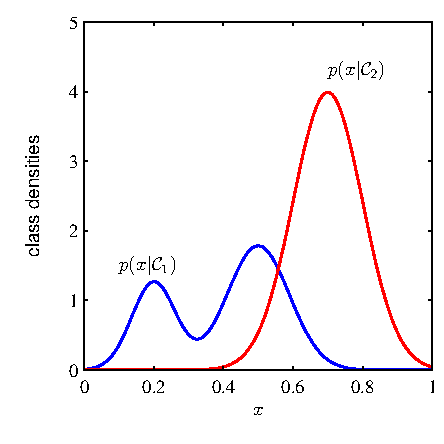
\includegraphics[width=.5\textwidth]{images/bishop-fig-1-27a.pdf}
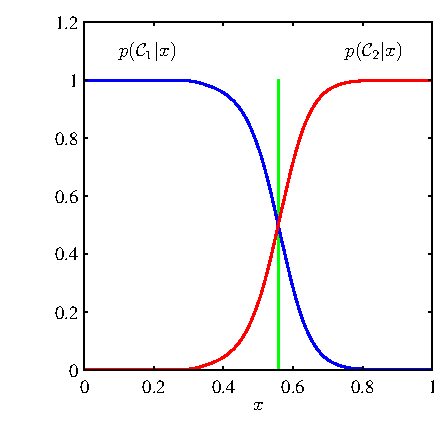
\includegraphics[width=.5\textwidth]{images/bishop-fig-1-27b.pdf}
\end{center}
\scriptsize {\bf Figure 1.27}
(\href{http://research.microsoft.com/en-us/um/people/cmbishop/prml}
{Bishop, 2006}): Example of the class-conditional densities for two
classes having a single input variable $x$ (left plot) together with
the corresponding posterior probabilities (right plot). Note that the
left-hand mode of the class-conditional density $p(x|C_1)$, shown in
blue on the left plot, has no effect on the posterior
probabilities. The vertical green line in the right plot shows the
decision boundary in $x$ that gives the minimum misclassification rate.
\end{frame}

\begin{frame}\frametitle{Why conditional models?}
\begin{itemize}
\item \url{https://class.coursera.org/nlp/lecture/131}  See the text
  classification example.
\item
  \url{http://www.cs.berkeley.edu/~klein/papers/maxent-tutorial-slides.pdf}
  See examples on sensors and stoplights.  ``Even with exactly the
  same features, changing from joint to conditional estimation
  increases performance.''  (Klein and Manning 2002, WSD using
  Senseval-1 data)
\end{itemize}
\end{frame}

\begin{frame}\frametitle{Conditional log-linear models: Likelihood}
\begin{itemize}
\item Represent $(x, y)$ pairs using a feature vector function
  $\vec{g}: \mathcal{X} \times \mathcal{Y} \rightarrow
  \mathbb{R}^d:$ \[
\vec{g}(x, y) = [ g_1(x, y), g_2(x, y), \dots, g_d(x, y) ]^T
\]
\item Define score as linear combination of feature values: \[
  \score(x, y) = \vec{w}^T \vec{g}(x, y) = \sum w_i g_i(x, y)
\]
\item Maximizing score equivalent to maximizing conditional log-linear
  likelihood:
\begin{eqnarray*}
  p_w(y|x) &=& \frac{1}{z_w(x)}\exp \vec{w}^T \vec{g}(x, y) \\
  z_w(x) &=& \sum_{y\in\mathcal{Y}} \exp \vec{w}^T \vec{g}(x, y) \\
  \argmax_{y\in\mathcal{Y}} p_w(y|x)
    &=& \argmax_{y\in\mathcal{Y}} \exp \vec{w}^T \vec{g}(x, y) \\
    &=& \argmax_{y\in\mathcal{Y}} \vec{w}^T \vec{g}(x, y)
\end{eqnarray*}
\end{itemize}
\end{frame}

\begin{frame}\frametitle{Conditional log-linear models: What features?}
A typical feature set for string classification (inspired by Naive
Bayes parameters):\begin{itemize}
\item One binary feature for each class:\[
g_j(x, y) = 
\begin{cases}
1,& \text{if } y=j \\
0,& \text{otherwise.}
\end{cases}
\]
\item One binary feature for each word-class pair:\[
g_{ij}(x, y) = 
\begin{cases}
1,& \text{if word}_i\in x, y=j \\
0,& \text{otherwise.}
\end{cases}
\]
\end{itemize}
Typically each feature should be sensitive to the class (a feature
that only looks at $x$ would not be useful in modeling $p(y|x)$), and
possibly some properties of the input string $x$.
\end{frame}

\begin{frame}\frametitle{Conditional log-linear models: maximum
    likelihood}
Given training data $\{(x_1, y_1), (x_2, y_2), \dots \}$, the
maximum likelihood estimation for weights $\vec{w}$: \begin{eqnarray*}
\vec{w}_\textsc{ml} &=& \argmax_\vec{w} \prod p_\vec{w}(y_i | x_i) \\
&=& \argmax_\vec{w} \sum \log p_\vec{w}(y_i | x_i) \\
&=& \argmax_\vec{w} \sum \vec{w}^T \vec{g}(x_i, y_i) - \log z_w(x_i)
\end{eqnarray*}
\begin{itemize}
\item There is no closed form solution.
\item The function is concave (unique maximum).
\item Algorithms like LBFGS can find the maximum quickly given the
  gradient.
\end{itemize}
\end{frame}

\begin{frame}\frametitle{Conditional log-linear models: Gradient}
\begin{eqnarray*}
\ell(\vec{w}) &=& \frac{1}{N} \sum_{i=1}^N \left[ \vec{w}^T
    \vec{g}(x_i, y_i) - \log z_w(x_i) \right] \\
\frac{\partial \ell(\vec{w})}{\partial w_j} &=& \frac{1}{N}
  \sum_{i=1}^N \left[ g_j(x_i, y_i) - \frac{\sum_{y\in\mathcal{Y}}
      g_j(x_i, y) \exp \vec{w}^T \vec{g}(x_i, y)}{z_w(x_i)}
    \right] \\
&=& \frac{1}{N} \sum_{i=1}^N \left[ g_j(x_i, y_i) -
    \sum_{y\in\mathcal{Y}} g_j(x_i, y) p_w(y|x_i) \right] \\
&=& \frac{1}{N} \sum_{i=1}^N \left[ g_j(x_i, y_i) -
    \mathbb{E}_{p_\vec{w}(Y|X)} g_j(x_i ,Y) \right] \\
&=& \mathbb{E}_{\tilde{p}(X,Y)} g_j(X,Y) -
  \mathbb{E}_{p_\vec{w}(X,Y)} g_j(X,Y)
\end{eqnarray*}
where $p_\vec{w}(X,Y) = \tilde{p}(X)p_\vec{w}(Y|X)$ and
$\tilde{p}$ denotes empirical distribution (i.e. data frequency).
\end{frame}

\begin{frame}\frametitle{Conditional log-linear models: Feature expectations}
\[
\mathbb{E}_{\tilde{p}(X,Y)} g_j(X,Y) =
  \mathbb{E}_{p_\vec{w}(X,Y)} g_j(X,Y)\quad \mbox{ at maximum.}
\]
\begin{itemize}
\item The first expectation is over the empirical distribution
  $\tilde{p}$.
\item The second expectation is over the model distribution $p_w$.
\item At the $\vec{w}$ that maximizes the likelihood, the model
  expectation of each feature is equal to the empirical expectation.
\end{itemize}
\end{frame}

\begin{frame}\frametitle{Conditional log-linear models: Logistic regression}
\begin{itemize}
\item General conditional log-linear model:\[
  p_\vec{w}(y|x) = \frac{\exp \vec{w}^T \vec{g}(x, y)}
  {\sum_{y\in\mathcal{Y}} \exp \vec{w}^T \vec{g}(x, y)}
\]
\item Logistic regression is the binary output case: $y\in\{+1,-1\}$ \[
  p_\vec{w}(y|x) = \frac{\exp \vec{w}^T \vec{g}(x, y)}
  {\exp \vec{w}^T \vec{g}(x, y)+\exp \vec{w}^T \vec{g}(x, -y)}
\]
\item Define $\vec{g}(\vec{x}, +1) = \vec{x}$ and $\vec{g}(\vec{x},
  -1) = \vec{0}$:
\begin{eqnarray*}
  p_\vec{w}(Y=+1|x) &=&
  \frac{\exp \vec{w}^T \vec{x}}
       {\exp \vec{w}^T \vec{x}+1} =
  \frac{1}{1+\exp(-\vec{w}^T \vec{x})} \\
  p_\vec{w}(Y=-1|x) &=&
  \frac{1}{\exp \vec{w}^T \vec{x}+1} \\
  p_\vec{w}(y|x) &=& 
  \frac{1}{1+\exp(-\vec{w}^T \vec{x} y)} \\
\end{eqnarray*}
\item Decision rule: $\argmax_y p_\vec{w}(y|x)=+1\Leftrightarrow\vec{w}^T\vec{x} > 0$.
\end{itemize}  
\end{frame}

\begin{frame}\frametitle{Log-linear models under other names}
\begin{itemize}
\item \textbf{Maximum entropy models:} When we represent data using a
  given set of features and ask for the probability distribution with
  maximum entropy consistent with empiricial feature expectations, the
  log-linear model gives the unique solution.  (Thus they are also
  called maximum entropy models.)
\item \textbf{Logistic regression:} (actually a classification, not a
  regression technique) is a conditional log-linear model for binary
  outputs.
\item \textbf{CRF, MEMM:} Structured conditional log-linear models (to
  be covered later).
\item \textbf{Naive Bayes:} gives the maximum likelihood solution to a
  {\em generative} log-linear model (modeling joint instead of
  conditional probability as a log-linear function of features)
  i.e. $p_\vec{w}(x,y) = \frac{1}{z_\vec{w}}\exp \vec{w}^T \vec{g}(x, y)$
  (see
  \href{http://www.denizyuret.com/2010/11/naive-bayes-is-joint-maximum-entropy.html}{my
    blog post on this}).
%% linear svm vs logistic regression with l1/l2 prior, l1/l2 loss?
\end{itemize}
\end{frame}

\begin{frame}\frametitle{Conditional log-linear models: Overfitting}
%% LSP pp.94
Example from
(\href{http://www.morganclaypool.com/doi/abs/10.2200/S00361ED1V01Y201105HLT013}{LSP},
pp.94): Consider a feature $g_6$ with value 1 on a single training
example $(x_9, y_9)$ and 0 for every other $(x, y)$ pair.  The
derivative of the log likelihood with respect to $w_6$
is: \begin{eqnarray*} \frac{\partial \ell(\vec{w})}{\partial w_6} &=&
  \frac{1}{N} \sum_{i=1}^N \left[ g_6(x_i, y_i) -
    \sum_{y\in\mathcal{Y}} g_6(x_i, y) p_\vec{w}(y|x_i) \right]
  \\ &=& \frac{1}{N} \left[g_6(x_9, y_9) - g_6(x_9, y_9)
    p_\vec{w}(y_9|x_9)\right] \\ &=& \frac{1}{N} \left[ 1 -
    p_\vec{w}(y_9|x_9) \right]
\end{eqnarray*}
This derivative can only approach 0 if $p_\vec{w}(y_9|x_9)$
approaches 1.\begin{eqnarray*}
p_\vec{w}(y_9|x_9) &=& \frac{\exp \vec{w}^T \vec{g}(x_9,y_9)}
{\sum_{y\in\mathcal{Y}} \exp \vec{w}^T \vec{g}(x_9,y)} \\
\end{eqnarray*}
This can only happen if $w_6\rightarrow\infty$ and for every feature
$g_j$ involving a competing $y$, $w_j\rightarrow-\infty$.
\end{frame}

\begin{frame}\frametitle{MAP estimation as a solution to overfitting}
\begin{itemize}
\item Predictive distribution (what we really want):\begin{eqnarray*}
  P(D'|D,\mathcal{H}) &=& \int P(D'|Q,\mathcal{H}) P(Q|D,\mathcal{H}) dQ 
%\\ \text{where } P(Q|D,\mathcal{H}) &\propto& P(D|Q,\mathcal{H}) P(Q|\mathcal{H})
\end{eqnarray*}
\item Maximum likelihood estimate (MLE):\begin{eqnarray*}
  P(D'|D,\mathcal{H}) &\approx& P(D'|Q_\text{ML}, \mathcal{H}) \\
\mbox{where } Q_\text{ML} &=& \argmax_Q P(D|Q,\mathcal{H})
\end{eqnarray*}
\item Maximum a-posteriori estimate (MAP):\begin{eqnarray*}
  P(D'|D,\mathcal{H}) &\approx& P(D'|Q_\text{MAP}, \mathcal{H}) \\
\mbox{where } Q_\text{MAP} &=& \argmax_Q P(Q|D,\mathcal{H}) \\
\mbox{ and } P(Q|D,\mathcal{H}) &\propto& P(D|Q,\mathcal{H}) P(Q|\mathcal{H})
\end{eqnarray*}
\end{itemize}
\footnotesize Note: $D'$ is future data, $D$ is past data,
$\mathcal{H}$ is the model and $Q$ its parameters.  In generative
models $D$ and $D'$ stand for both the input $X$ and the output $Y$.
In conditional models they stand for the output $Y$ only.  The input
$X$ is assumed given ($X$ is on the condition (right) side of each
probability).
% expression, next to $\mathcal{H}$).
\end{frame}

\begin{frame}\frametitle{Conditional log-linear models: Gaussian MAP} %% LSP 94-97
Gaussian prior (aka L2 regularization):\begin{eqnarray*}
p(\vec{w}|\mathcal{H}_G) &=& \prod_{j=1}^d \frac{1}{\sigma \sqrt{2\pi}}
\exp -\frac{w_j^2}{2\sigma^2} \\
\vec{w}_\text{MAP} &=& \argmax_\vec{w}\, \log p(D|\vec{w},\mathcal{H}_G)
+ \log p(\vec{w}|\mathcal{H}_G) \\
&=& \argmax_\vec{w}\, \ell(\vec{w}) -\frac{1}{2\sigma^2}\sum w_j^2 \\
&=& \argmax_\vec{w}\, \ell(\vec{w}) - \frac{\lambda}{2}\|\vec{w}\|_2^2 \quad\text{where }\lambda=\frac{1}{\sigma^2}
\end{eqnarray*}
\end{frame}
\begin{frame}\frametitle{Conditional log-linear models: Laplacian MAP} %% LSP 94-97
Laplacian prior (aka L1 regularization):\begin{eqnarray*}
p(\vec{w}|\mathcal{H}_L) &=& \prod_{j=1}^d \frac{1}{2b} \exp -\frac{|w_j|}{b}\\
\vec{w}_\text{MAP} &=& \argmax_\vec{w}\, \log p(D|\vec{w},\mathcal{H}_L)
+ \log p(\vec{w}|\mathcal{H}_L) \\
&=& \argmax_\vec{w}\, \ell(\vec{w}) -\frac{1}{b}\sum |w_j| \\
&=& \argmax_\vec{w}\, \ell(\vec{w}) - \lambda \|\vec{w}\|_1 \quad\text{where }\lambda=\frac{1}{b}
\end{eqnarray*}
\end{frame}

\begin{frame}\frametitle{Conditional log-linear models: L1 vs. L2} %% Hastie
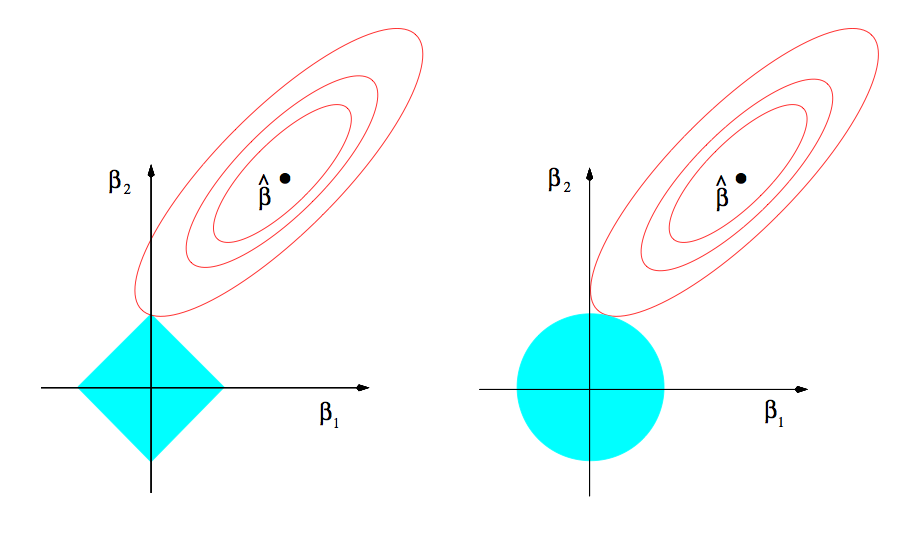
\includegraphics[width=.9\textwidth]{images/hastie-fig-3-11.png}

\footnotesize {\bf Figure 3.11}
(\href{http://www-stat.stanford.edu/~tibs/ElemStatLearn}{Hastie et
  al. 2009}): $\beta_1$ and $\beta_2$ are model parameters,
$\hat{\beta}$ is the ML estimate, the red ellipses are likelihood
contours, and the solid blue shapes are the L1 (left) and L2 (right)
prior contours.  The L1 prior results in a more {\bf sparse} (with
lots of zeros) parameter vector.  The L2 prior pushes many parameters
close to zero but does not quite get rid of them.
\end{frame}

\section{Non-probabilistic models}
\frame{\sectionpage}

\begin{frame}\frametitle{A non-probabilistic view of learning} %% LSP 98-100
\begin{itemize}
\item An alternative view of machine learning replaces probabilistic
  inference with the minimization of a {\bf loss
    function}\footnote{There is quite a bit of confusing terminology
    in the literature: the loss is also referred to as the cost,
    error, or regret and its negative as reward, utility, or the
    objective function.}.
\item Let $\mathcal{H}$ denote the set of all possible predictors that
  map $\mathcal{X}\rightarrow\mathcal{Y}$.  The loss for
  $h\in\mathcal{H}$ is a measurement of the badness of the predictor
  $h$ given input $x$ when $y$ is the correct output:
  \[ \loss(x, y; h) \in \mathcal{X} \times \mathcal{Y}
  \times (\mathcal{X}\rightarrow\mathcal{Y}) \rightarrow \mathbb{R}
\]
\item Given $\mathcal{H}$ and $\loss$, the learning problem becomes:\[
  \argmin_{h\in\mathcal{H}} \mathbb{E}[\loss(X, Y; h)] +
  \textit{model-complexity}(h)
\]
\item The first term (expected loss) is known as the {\bf
  risk}\footnote{The risk is typically estimated using training data
  in which case it is known as the {\bf empirical risk}:
  $\mathbb{E}[\loss(X, Y; h)] \approx \frac{1}{N} \sum_{i=1}^N
  \loss(x_i, y_i; h)$ }, and the second term is called the {\bf
  regularization} term\footnote{The regularization term serves the
  same function as the prior in MAP.}.
\end{itemize}
\end{frame}

\begin{frame}\frametitle{Probabilistic inference $\rightarrow$ log loss}
The probabilistic learning methods we have covered can be restated in
terms of loss functions.
\begin{itemize}
\item Maximizing log likelihood in generative models can be seen as
  minimizing the {\bf log loss}:\[
\loss(x, y; h) = -\log p(x, y | h)
\]
\item Maximizing log likelihood in conditional models gives another
  form of {\bf log loss}:\[
\loss(x, y; h) = -\log p(y | x, h)
\]
\item Variants of {\bf log loss} for conditional log-linear models and
  logistic regression: \begin{eqnarray*}
\loss_{LL}(\vec{x}_i, y_i; \vec{w}) &=& 
-\vec{w}^T \vec{g}(\vec{x}_i,y_i) 
+\log \sum_{y\in\mathcal{Y}} \exp \vec{w}^T \vec{g}(\vec{x}_i,y) \\
\loss_{LR}(\vec{x}_i, y_i; \vec{w}) &=& \log(1 + \exp(-\vec{w}^T\vec{x}_i y_i))
\end{eqnarray*}
\end{itemize}
\end{frame}

\begin{frame}\frametitle{Logistic regression log-loss as a function of $\vec{w}^T\vec{x}y$}
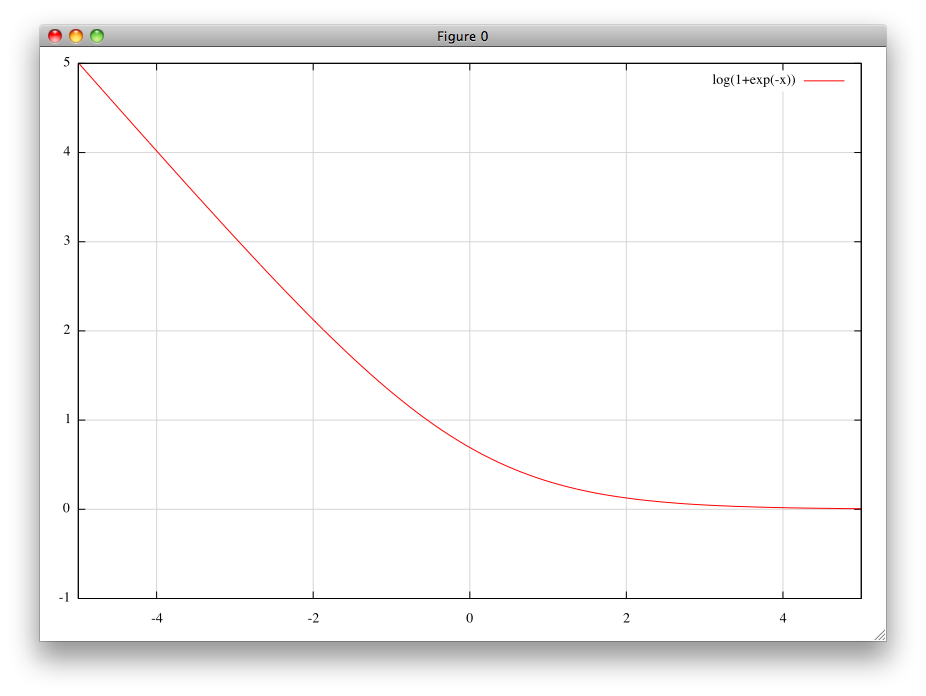
\includegraphics[width=\textwidth]{images/log-loss.png}
\end{frame}

\begin{frame}\frametitle{MAP prior $\rightarrow$ regularization term}
\begin{itemize}
\item Gaussian prior is equivalent to L2 regularization: \[
  \argmin_\vec{w}\, \frac{1}{N} \sum_{i=1}^N -\log p(y_i|x_i,\vec{w}) + \frac{\lambda}{2}\|\vec{w}\|_2^2
\]
\item Laplacian prior is equivalent to L1 regularization: \[
  \argmin_\vec{w}\, \frac{1}{N} \sum_{i=1}^N -\log p(y_i|x_i,\vec{w}) + \lambda \|\vec{w}\|_1
\]
\end{itemize}
\end{frame}

\begin{frame}\frametitle{Potential problems with log loss}
\begin{eqnarray*}
\loss(x, y; h) &=& -\log p(x, y | h)\quad\text{or}\\
\loss(x, y; h) &=& -\log p(y | x, h)
\end{eqnarray*}
\begin{itemize}
\item Even if the model correctly predicts $y_i$ as the most probable
  output for $x_i$, there is still pressure to diminish the loss
  function as long as other $y\in\mathcal{Y}$ have non-zero
  probability.
\item Not all alternative $y\in\mathcal{Y}$ may be equally bad, some
  wrong answers may be preferrable to others.  This is not represented
  in log loss.\footnote{To be more accurate, probabilistic models
    separate inference and decision.  Probabilities are used to assign
    likelihoods to various states of nature and decision theory is
    used to take the optimal action under these likelihoods.
    Non-probabilistic models try to solve both inference and decision
    using a single optimization.  See 
    \href{http://research.microsoft.com/en-us/um/people/cmbishop/prml}{Bishop
      2006} Sec. 1.5, \href{http://www.cs.ubc.ca/~murphyk/MLbook}{Murphy
      2012} Sec. 5.7, 6.3, 6.5 for more detailed discussions.
  }
\end{itemize}
\end{frame}


\begin{frame}\frametitle{Perceptron Algorithm 
(\href{http://www2.denizyuret.com/bibtex.php?fn=show&nselect=1&e1=986}{Rosenblatt 1958})}
Initialize $\vec{w} \leftarrow \vec{0}$\\
For pass $t=1\dots T$, example $i=1\dots N$:\\
\begin{itemize}
\item Predict $\hat{y}_i\in\{-1,+1\}$:
\[
\hat{y}_i \leftarrow \begin{cases}
+1,& \text{if } \vec{w}^T \vec{x}_i > 0\\
-1,& \text{otherwise.}
\end{cases}
\]
{\small (Note that the prediction rule is the same as logistic regression.)}
\item Update $\vec{w}$ if you made a mistake:
\[\vec{w} \leftarrow \vec{w} 
+ \vec{x}_i y_i
\quad\text{ if } \hat{y}_i \neq y_i
\]
\end{itemize}
\end{frame}


\begin{frame}\frametitle{Perceptron Algorithm: example run}
\begin{columns}
\column{.66\textwidth}
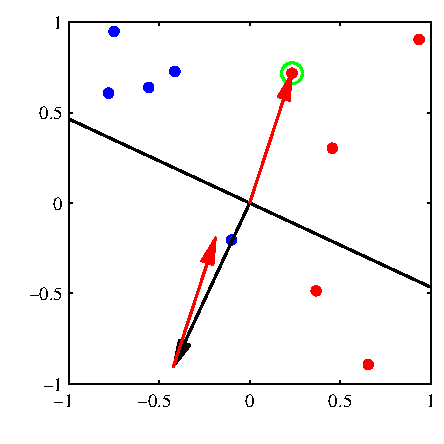
\includegraphics[height=.4\textheight]{images/bishop-fig-4-7a.pdf}
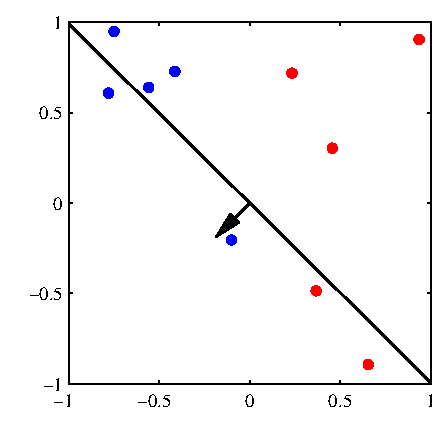
\includegraphics[height=.4\textheight]{images/bishop-fig-4-7b.pdf}\\ 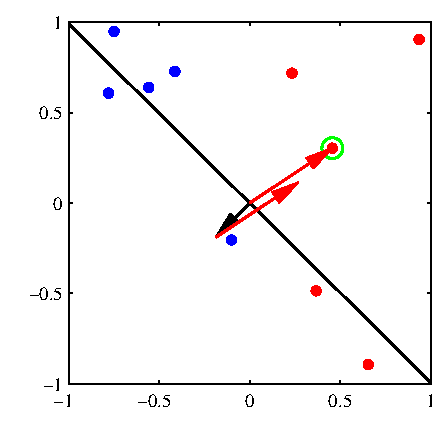
\includegraphics[height=.4\textheight]{images/bishop-fig-4-7c.pdf}
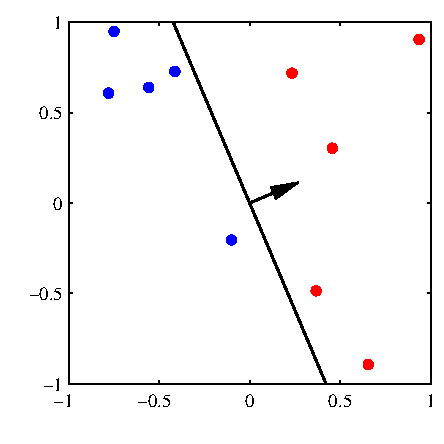
\includegraphics[height=.4\textheight]{images/bishop-fig-4-7d.pdf}
\column{.33\textwidth}\footnotesize {\bf Figure 4.7}
(\href{http://research.microsoft.com/en-us/um/people/cmbishop/prml}{Bishop
  2006}): Example run of the perceptron algorithm, showing data points
from two classes: red (+1) and blue (-1) in a 2D feature space. The
parameter vector $\vec{w}$ is shown as a black arrow together with the
corresponding decision boundary (black line), in which the arrow
points towards the decision region which classified as belonging to
the red class.
\end{columns}
\end{frame}


\begin{frame}\frametitle{Perceptron Algorithm: geometry}
\begin{columns}
\column{.65\textwidth}
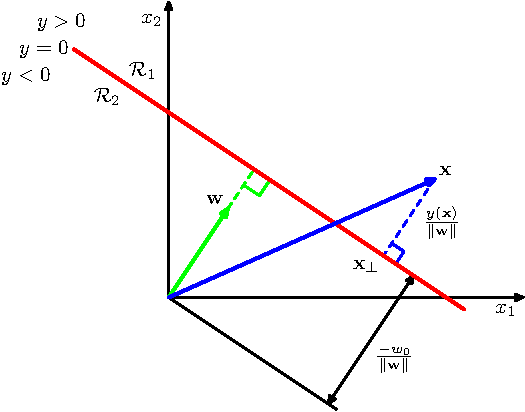
\includegraphics[width=\textwidth]{images/bishop-fig-4-1.pdf}
\column{.35\textwidth}\footnotesize {\bf Figure 4.1}
(\href{http://research.microsoft.com/en-us/um/people/cmbishop/prml}{Bishop
  2006}): Geometry of a binary perceptron with two dimensional input.
The output is $+1$ if $y(\vec{x})=\vec{w}^T\vec{x}+w_0 > 0$ and $-1$
otherwise (the bias term $w_0$ has been made explicit).  The decision
surface, shown in red, is perpendicular to $\vec{w}$, and its
displacement from the origin is controlled by the bias parameter
$w_0$. Also, the signed orthogonal distance of a general point
$\vec{x}$ from the decision surface (margin) is given by
$y(\vec{x})/\|w\|$.
\end{columns}
\end{frame}


\begin{frame}\frametitle{What does the perceptron optimize?}
\begin{itemize}
\item We typically represent a predictor $h$ in terms of some parameters
  $\vec{w}$ and search for $\vec{w}$ that minimize empirical
  risk: \[ 
  \argmin_\vec{w} \sum_{i=1}^N \loss(x_i, y_i; \vec{w})
  \]
\item {\bf Gradient descent} can be used when no closed form solution
  is available (however, beware of local minima): \[ \vec{w} \leftarrow
  \vec{w} - \alpha \sum_{i=1}^N \nabla \loss(x_i, y_i; \vec{w})
\]
\item {\bf
  \href{http://en.wikipedia.org/wiki/Stochastic_gradient_descent}
       {Stochastic gradient descent}} approximates the true gradient 
  of the loss by a gradient at a single example: \[ \vec{w}
  \leftarrow \vec{w} - \alpha\, \nabla \loss(x_i, y_i; \vec{w})
\]
\end{itemize}
\end{frame}


\begin{frame}\frametitle{Perceptron Algorithm: loss function}
\begin{itemize}
\item The perceptron update rule:
\[
\vec{w} \leftarrow \vec{w} 
+ \vec{x}_i y_i
\quad\text{ if } \hat{y}_i \neq y_i
\]
\item can be seen as performing stochastic gradient descent of the
  following loss function:
\[
\loss_P(x_i, y_i; \vec{w}) = \begin{cases}
-\vec{w}^T\vec{x}_i y_i,& \text{if } \vec{w}^T\vec{x}_i y_i<0 \\
0,& \text{otherwise.}
\end{cases}
\]
\item Compare this with log-loss from logistic regression: \[
  \loss_{LR}(x_i, y_i; \vec{w}) = \log(1 + \exp(-\vec{w}^T\vec{x}_i y_i))
\]
\end{itemize}
\end{frame}

\begin{frame}\frametitle{Perceptron vs. log-loss as a function of
    $\vec{w}^T\vec{x} y$}
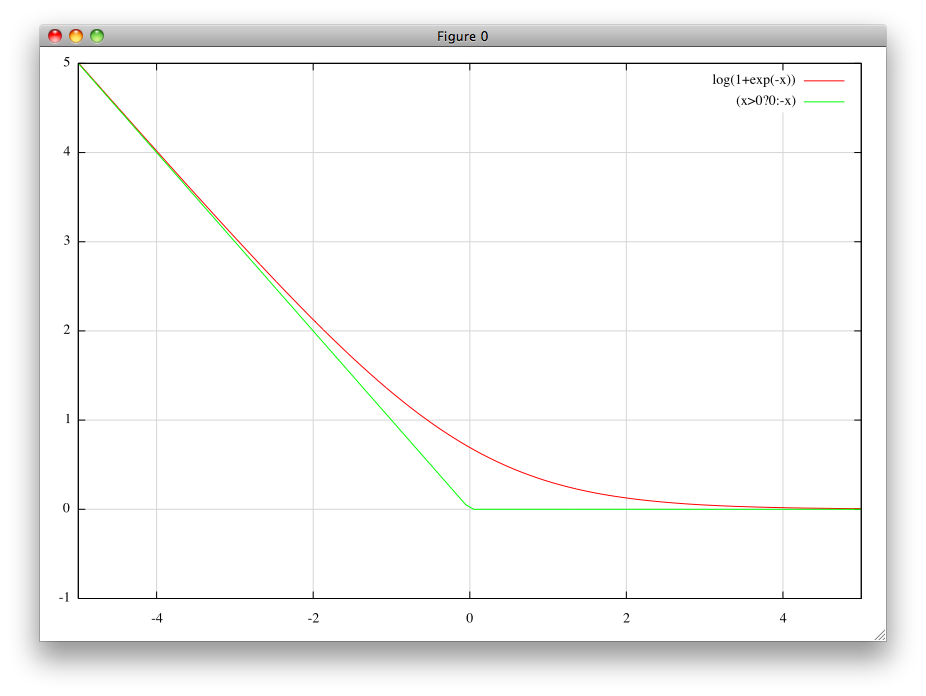
\includegraphics[width=\textwidth]{images/perceptron-loss.png}
\end{frame}


\begin{frame}\frametitle{Multiclass Perceptron
(\href{http://aclweb.org/anthology//W/W02/W02-1001.pdf}{Collins 2002})} %% LSP 101-103
Initialize $\vec{w} \leftarrow \vec{0}$\\
For pass $t=1\dots T$, example $i=1\dots N$:\\
\begin{itemize}
\item $\hat{y}_i \leftarrow \argmax_{y\in\mathcal{Y}}
    \vec{w}^T\vec{g}(\vec{x}_i, y)$
\item $\vec{w} \leftarrow \vec{w} 
+\vec{g}(\vec{x}_i,y_i)
-\vec{g}(\vec{x}_i,\hat{y}_i)$ 
\hspace{10mm}
\small (No update if $\hat{y}_i=y_i$.)
\end{itemize}
\vspace{20mm}
Note that we can recover the binary perceptron algorithm if we set
$\vec{g}(\vec{x},+1)=\vec{x}$ and $\vec{g}(\vec{x},-1)=\vec{0}$.
\end{frame}

\begin{frame}\frametitle{Multiclass Perceptron: loss function}
\begin{itemize}
\item {\bf Perceptron update rule:}
\[ \vec{w} \leftarrow \vec{w} 
+\vec{g}(x_i,y_i)
-\vec{g}(x_i,\hat{y}_i)
\]
\item {\bf Perceptron criterion (loss function):} This update rule can
  be interpreted as {\bf stochastic gradient descent}
  on the following loss function:
% (negative of margin for wrong outputs, 0 for correct ones):
% (a variant of hinge loss with the hinge at origin): 
\[
\loss_P(x_i, y_i; \vec{w}) = 
-\vec{w}^T \vec{g}(x_i,y_i)
+\max_{y\in\mathcal{Y}} \vec{w}^T \vec{g}(x_i,y)
\]

\item Compare this with log-loss from conditional log-linear models: \[
\loss_{LL}(x_i, y_i; \vec{w}) = 
-\vec{w}^T \vec{g}(x_i,y_i) 
+\log \sum_{y\in\mathcal{Y}} \exp \vec{w}^T \vec{g}(x_i,y) 
\]

\item Note that log-sum-exp is a smooth approximation to the maximum
  function.
% \item Compare the loss in binary case with the ones in Figure 7.5.
\end{itemize}
\end{frame}

\begin{frame}\frametitle{Perceptron Algorithm: convergence theorem}
{\bf Perceptron convergence theorem:} The perceptron algorithm will
find $\vec{w}$ with zero error on training set after a finite number
of mistakes if one exists!
\vspace{5mm}

A training set $\{(x_1,y_1),\dots,(x_N,y_N)\}$ with diameter $R$ is
separable with margin $\delta$ if there is a $\vec{w}_*$ with
$\|\vec{w}_*\|=1$ such that: \begin{eqnarray*}
  \vec{w}_*^T\vec{g}(\vec{x}_i,y_i) - \vec{w}_*^T\vec{g}(\vec{x}_i,\bar{y}_i)
  &>& \delta \quad\text{and}\\ \|\vec{g}(\vec{x}_i, y_i) -
  \vec{g}(\vec{x}_i, \bar{y}_i)\| &<& R
\end{eqnarray*}
for all $i \in \{1,\dots,N\}$ and $\bar{y}_i \in \bar{\mathcal{Y}_i}$ where
$\bar{\mathcal{Y}_i}$ is the set of {\bf incorrect} outputs and $y_i$
is the correct output for $\vec{x}_i$.  In such a training set, the
number of mistakes $K$ made by the perceptron algorithm is bounded
by: \[ K \leq \frac{R^2}{\delta^2}
\]
\end{frame}

\begin{frame}\frametitle{Perceptron Algorithm: convergence proof}
\small
\begin{itemize}
\item Let $\vec{w}_k$ be the weights before the $k$'th mistake.
  ($\vec{w}_1 = \vec{0}$).
\item Let $i$ be the example where the $k$'th mistake is made, and
  $\hat{y}_i = \argmax_{y\in\mathcal{Y}} \vec{w}_k^T \vec{g}(\vec{x}_i,y)$
  the incorrect answer given.
\item After the update: $\vec{w}_{k+1} = \vec{w}_k + \vec{g}(\vec{x}_i,y_i) -
  \vec{g}(\vec{x}_i,\hat{y}_i)$
\item Dot product the update with $\vec{w}_*$ to get a lower bound on
  $\|\vec{w}_{k+1}\|$ :\begin{eqnarray*} 
\vec{w}_*^T \vec{w}_{k+1} &=& \vec{w}_*^T \vec{w}_k + \vec{w}_*^T
  \vec{g}(\vec{x}_i,y_i) - \vec{w}_*^T \vec{g}(\vec{x}_i,\hat{y}_i) \\
 &\geq& \vec{w}_*^T \vec{w}_k + \delta \\
 &\geq& k \delta 
  \quad\text{because } \vec{w}_1=\vec{0} \\
\|\vec{w}_{k+1}\| &\geq& k \delta 
  \quad\text{because } \|\vec{w}_*\|=1
\end{eqnarray*} 
\item Square the update to get an upper bound on
  $\|\vec{w}_{k+1}\|$: \begin{eqnarray*}
\|\vec{w}_{k+1}\|^2 &=& \|\vec{w}_k\|^2 + \|\vec{g}(\vec{x}_i,y_i) -
  \vec{g}(\vec{x}_i,\hat{y}_i)\|^2 \\
  && +\, 2 \vec{w}_k^T (\vec{g}(\vec{x}_i,y_i) -
  \vec{g}(\vec{x}_i,\hat{y}_i)) \\
&\leq& \|\vec{w}_k\|^2 + \|\vec{g}(\vec{x}_i,y_i) -
  \vec{g}(\vec{x}_i,\hat{y}_i)\|^2 \\
&\leq& \|\vec{w}_k\|^2 + R^2 \leq k R^2
\end{eqnarray*}
\item Combining the two inequalities gives: $ k^2 \delta^2 \leq k R^2
  \Rightarrow k \leq R^2 / \delta^2 $
\end{itemize}
\end{frame}

\begin{frame}\frametitle{Perceptron Algorithm: margin and robustness}
\begin{center}
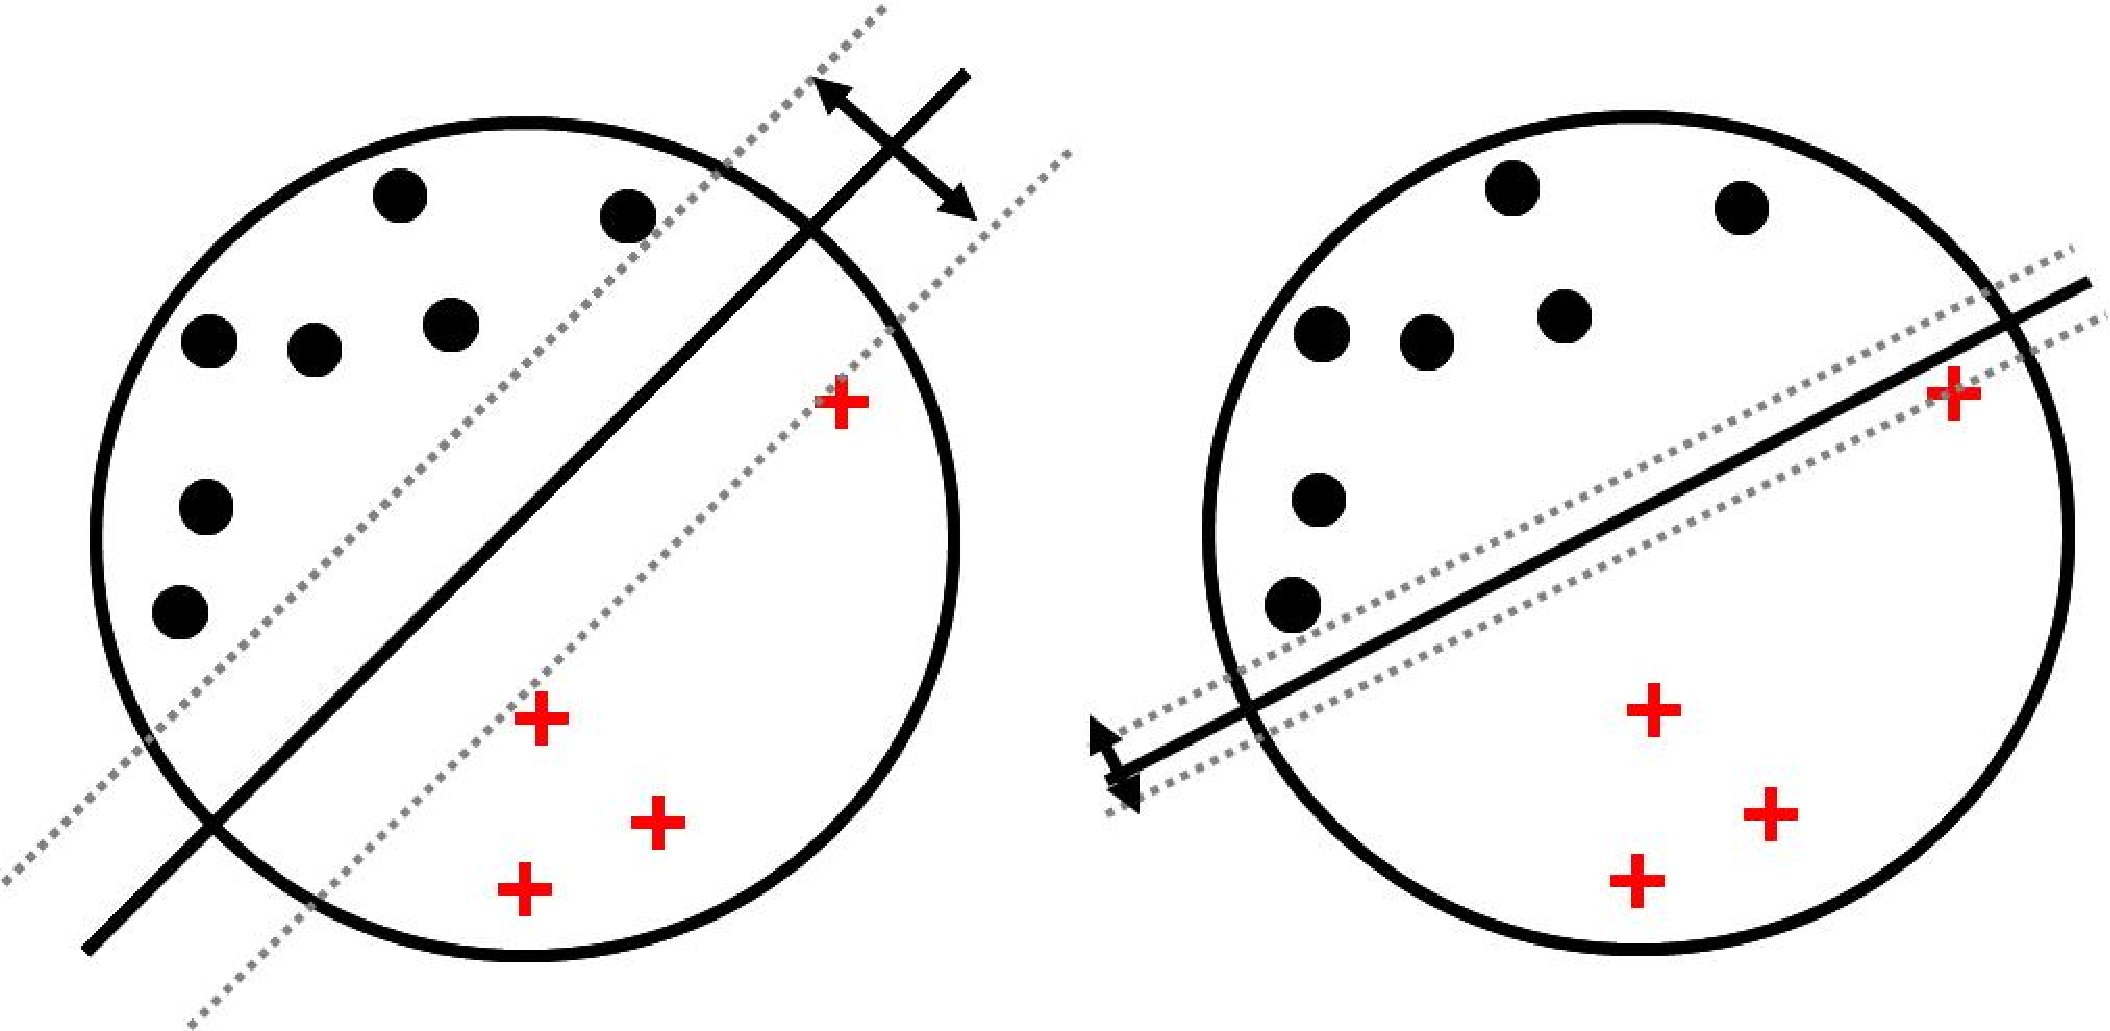
\includegraphics[width=\textwidth]{images/largeMarginPrinciple2.pdf}
\end{center}\footnotesize
{\bf Figure 14.11} (\href{http://www.cs.ubc.ca/~murphyk/MLbook}{Murphy
  2012}): The perceptron algorithm finds an arbitrary separating
boundary if there is one and stops updating afterwards.  If there is
no separating boundary it may oscillate between different solutions.
Different ways of making the perceptron more robust include {\bf voting},
{\bf averaging}, and {\bf early stopping} (see
\href{http://aclweb.org/anthology//W/W02/W02-1001.pdf}{Collins 2002}).
Another alternative is to search for the solution with the {\bf
  maximum margin} (which leads us to SVMs).
\end{frame}

\begin{frame}\frametitle{Introducing margin}
\begin{itemize}
\item Let $\delta(\vec{w},\vec{x}_i)$ be the difference between the
  score of the correct output and the closest incorrect output for
  input $\vec{x}_i$:
\[
  \delta(\vec{w}, \vec{x}_i) =
  \vec{w}^T\vec{g}(\vec{x}_i,y_i) - \max_{\bar{y}_i \in 
    \bar{\mathcal{Y}_i}} \vec{w}^T\vec{g}(\vec{x}_i,\bar{y}_i)
\]
where $\bar{\mathcal{Y}_i}$ is the set of incorrect outputs for $x_i$.
\item Note that in the binary case (i.e. $y_i\in\{-1,+1\}$) using 
$\vec{g}(\vec{x},+1)=\vec{x}$ and $\vec{g}(\vec{x},-1)=\vec{0}$,
$\delta$ becomes:
\[
  \delta(\vec{w}, \vec{x}_i) = \vec{w}^T\vec{x}_i y_i
\]
\item Different multiples of $\vec{w}$ will give different scores but
  will have the same decision boundaries.  We normalize $\delta$ and
  define {\bf margin} as:
\[
  \text{margin}(\vec{w},\vec{x}_i) = \frac{\delta(\vec{w},\vec{x}_i)}{\|\vec{w}\|}
\]
\end{itemize}
\end{frame}


\begin{frame}\frametitle{Maximizing margin}
\begin{itemize}
\item To make the classifier more robust, we can find the $\vec{w}_*$
  that maximizes the margin of the point(s) closest to the boundary: 
\[
  \vec{w}_* = \argmax_\vec{w} \min_i \frac{\delta(\vec{w},\vec{x}_i)}{\|\vec{w}\|} 
\]
\item The solution is not unique; any multiple of $\vec{w}$ will have
  the same decision boundaries and the same margins as $\vec{w}$.
\item We can pick the max-margin $\vec{w}$ of unit length: \[
\vec{w}_* = \argmax_\vec{w}\; \min_i \delta(\vec{w},\vec{x}_i)
\;\text{s.t. } \|\vec{w}\|=1
\]
\item Or the one that makes the minimum score difference = 1: \[
\vec{w}_* = \argmax_\vec{w}\; \frac{1}{\|\vec{w}\|}
\;\text{s.t. } \min_i \delta(\vec{w},\vec{x}_i) = 1
\]
or equivalently: \[
\vec{w}_* = \argmin_\vec{w}\; \frac{1}{2} \|\vec{w}\|^2
\;\text{s.t. } \forall i, \delta(\vec{w},\vec{x}_i) \geq 1
\]
\end{itemize}
% - ok, this is bull shit
% - why is maximizing the margin mean making it bigger than 1?  it doesn't.
% > actually it doesn't have to be 1, any finite value will do.
% - we are not maximizing margin (don't care once a point is past 1)
% but minimizing finite margin violations?
% > yes, ``margin violations'' as a surrogate for number of mistakes.
% - need to understand this common optimization trick. done.
% > everything comes out of any multiple of w being the same.
% - there are two things going on here.  slack variables allow
% non-separable (or give difft solns even if separable).  slack does
% not start from 0 but 1 (or what LSP calls the cost).
% - slack variables change the problem from max-margin to something
% totally different.
% > not quite, minimizing slack is a surrogate for minimizing mistakes.
\end{frame}

\begin{frame}\frametitle{Introducing slack: SVM}
The optimization problem: 
\[
\vec{w}_* = \argmin_\vec{w}\; \frac{1}{2} \|\vec{w}\|^2
\;\text{s.t. } \forall i, \delta(\vec{w},\vec{x}_i) \geq 1
\]
will have no solutions if the data is not separable.  {\bf Support
  vector machines} introduce {\bf slack variables} $\xi_i \geq 0$ to
allow some points to violate the margin:
\[ 
\forall i, \delta(\vec{w},\vec{x}_i) \geq 1 - \xi_i
\]
and minimize a linear combination of the weight norm and margin
violations:
\[
\min_{\vec{w},\xi_i\geq 0}\; \frac{\lambda}{2} \|\vec{w}\|^2
+ \frac{1}{N} \sum_{i=1}^N \xi_i
\quad\text{s.t. }
\forall i, \delta(\vec{w},\vec{x}_i) \geq 1 - \xi_i
\]
\end{frame}

\begin{frame}\frametitle{Geometry of slack variables} %% LSP 103-104
%% \begin{itemize}
%% \item If the data is not separable we may need to allow some points to
%%   be misclassified.
%% \item We introduce a slack variable $\xi_i$ for each data point
%%   $(\mathbf{x}_i,y_i)$ defined as: \[
%%   \xi_i = \max(0, 1-\mathbf{w}^T\mathbf{x_i}y_i)
%% \]
%% \end{itemize}
\begin{center}
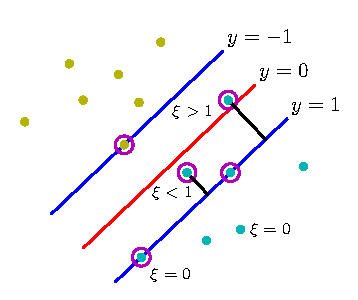
\includegraphics[height=.6\textheight]{images/bishop-fig-7-3.pdf}
\end{center}
\footnotesize {\bf Figure 7.3}
(\href{http://research.microsoft.com/en-us/um/people/cmbishop/prml}{Bishop
  2006}): The red line is the boundary, the blue lines are the margins
and $y=\mathbf{w}^T\mathbf{x}$ in the figure.  Note that $\xi_i=0$ if
$x_i$ is on the right side of the margin, $0<\xi_i\leq 1$ if $x_i$ is
on the wrong side of the margin but the right side of the boundary,
and $\xi_i > 1$ if $x_i$ is on the wrong side of the boundary.
\end{frame}

\begin{frame}\frametitle{Comparison of loss functions} %% LSP 103-104
\small
\begin{itemize}
\item Define $\delta_i = \vec{w}^T\vec{x}_i y_i$.
\item The hard margin optimization can be equivalently stated as: \[
% \vec{w}_* = \argmin_\vec{w}\frac{1}{2}\|\vec{w}\|^2
%\quad\text{such that } \forall i ,\; \vec{w}^T\vec{x}_i y_i \geq 1
  \vec{w}_* = \argmin_\vec{w} \sum_{i=1}^N E_\infty(\delta_i) + \frac{\lambda}{2} \|\vec{w}\|^2
\quad\text{where }
E_\infty(\delta)=\begin{cases}
0,& \text{if } \delta \geq 1 \\
\infty,& \text{otherwise.}
\end{cases}
\]
\item The soft margin optimization can be stated as: \[
  \vec{w}_* = \argmin_\vec{w} \sum_{i=1}^N E_{SV}(\delta_i) + \frac{\lambda}{2} \|\vec{w}\|^2
\quad\text{where }
E_{SV}(\delta)=\begin{cases}
0,& \text{if } \delta \geq 1 \\
1-\delta,& \text{otherwise.}
\end{cases}
\]
\item Compare this to logistic regression with a Gaussian prior: \[
  \vec{w}_* = \argmin_\vec{w} \sum_{i=1}^N E_{LR}(\delta_i) + \frac{\lambda}{2} \|\vec{w}\|^2
\quad\text{where }
E_{LR}(\delta) = \log(1 + \exp(-\delta))
\]
\item Compare this with unregularized marginless perceptron: \[
  \vec{w}_* = \argmin_\vec{w} \sum_{i=1}^N E_P(\delta_i)
\quad\text{where }
E_{P}(\delta)=\begin{cases}
0,& \text{if } \delta \geq 0 \\
-\delta,& \text{otherwise.}
\end{cases}
\]
\end{itemize}
\end{frame}

\begin{frame}\frametitle{Comparison of loss functions}
\begin{center}
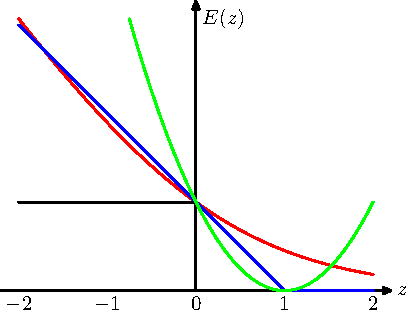
\includegraphics[height=.5\textheight]{images/bishop-fig-7-5.pdf}
\end{center}\footnotesize
{\bf Figure 7.5}
(\href{http://research.microsoft.com/en-us/um/people/cmbishop/prml}
{Bishop, 2006}): Loss functions for binary classification $y=\pm 1$.
$z=\mathbf{w}\mathbf{x}y$ and $E(z)$ is the error function for a
single instance.  The red curve is the {\bf log-loss} of logistic
regression, the black curve is the {\bf 0-1 loss}, the blue curve is
{\bf hinge loss} (used by SVM), and the green curve is the {\bf
  squared error} loss (used in regression).  Each loss function may
imply different optimum parameters for a given model.
\end{frame}


\begin{frame}\frametitle{Introducing cost: Structural SVM}
\begin{itemize}
\item Instead of requiring a minimum score difference of 1:
\[
  \vec{w}^T\vec{g}(\vec{x}_i,y_i) -
  \vec{w}^T\vec{g}(\vec{x}_i,\bar{y}_i) \geq 1\quad
  \forall \bar{y}_i \in \bar{\mathcal{Y}_i}
\]
\item We could require larger margins for worse answers\footnote{
  \href{http://www.morganclaypool.com/doi/abs/10.2200/S00361ED1V01Y201105HLT013}{LSP}
  calls this ``cost''}: \[
  \vec{w}^T\vec{g}(\vec{x}_i,y_i) -
  \vec{w}^T\vec{g}(\vec{x}_i,y) \geq \delta_0(\vec{x}_i,y,y_i)\quad
  \forall y \in \mathcal{Y}
\]
\item Minimizing margin violations: \[
\min_\vec{w}\; 
 \frac{\lambda}{2} \|\vec{w}\|^2
+ \frac{1}{N} \sum_{i=1}^N 
-  \vec{w}^T\vec{g}(\vec{x}_i,y_i) + \max_{y\in\mathcal{Y}}
(  \vec{w}^T\vec{g}(\vec{x}_i,y) + \delta_0(\vec{x}_i,y,y_i))
\]
\item Note that this is equivalent to the standard SVM when
  $\delta_0(\vec{x}_i,y,y_i)=[y\neq y_i]$\footnote{
  \href{http://en.wikipedia.org/wiki/Iverson_bracket}{Iverson bracket}
  notation: $[P]=1$ if $P$ is true and 0 otherwise.}.
\end{itemize}
\end{frame}

\begin{frame}\frametitle{Structural SVM vs. Conditional log-linear models}
\begin{itemize}
\item Compare the structural SVM objective: \[
\min_\vec{w}\; 
 \frac{\lambda}{2} \|\vec{w}\|^2
+ \frac{1}{N} \sum_{i=1}^N 
-  \vec{w}^T\vec{g}(\vec{x}_i,y_i) + \max_{y\in\mathcal{Y}}
(  \vec{w}^T\vec{g}(\vec{x}_i,y) + \delta_0(\vec{x}_i,y,y_i))
\]
\item to a conditional log-linear model with a Gaussian prior: \[
\min_\vec{w}\;
 \frac{\lambda}{2} \|\vec{w}\|^2
+ \frac{1}{N} \sum_{i=1}^N 
-\vec{w}^T \vec{g}(x_i,y_i) 
+\log \sum_{y\in\mathcal{Y}} \exp \vec{w}^T \vec{g}(x_i,y) 
\]
\item and to the perceptron loss function: \[
\min_\vec{w}\;
\frac{1}{N} \sum_{i=1}^N 
-\vec{w}^T \vec{g}(x_i,y_i)
+\max_{y\in\mathcal{Y}} \vec{w}^T \vec{g}(x_i,y)
\]
\end{itemize}
\end{frame}

\section{Unsupervised models}
\frame{\sectionpage}

\begin{frame}\frametitle{Unsupervised learning}
\begin{itemize}
\item The supervised methods we have seen so far learn to predict an
  output $y$ given an input $x$ from a training set with $(x, y)$
  input-output pairs.
\item Unsupervised methods learn to predict an output $y$ given an
  input $x$ without observing any $(x, y)$ examples, just from a
  training set of $x$'s!
\item {\sl But how can you learn anything about $y$'s without having
  any information about $y$'s?} you may naturally ask...
\item Even though we do not observe any $y$ examples, we do have
  information about $y$'s and how they relate to $x$'s in our
  hypothesized model, e.g. in the form of $p(x,y|w)$ for a
  generative model.
\item Question: why would one ever want to do this?
\end{itemize}
\end{frame}

\begin{frame}\frametitle{Unsupervised generative models}
\begin{itemize}
\item For supervised generative models we maximized log-likelihood: \[
  \argmax_w \sum_i \log p(x_i, y_i|w)
\]
\item But if we just observe $x$'s maximizing log-likelihood means: \[
  \argmax_w \sum_i \log p(x_i|w)
\]
\item For unsupervised learning, we can incorporate the $y$'s in the
  model (expressing information about how they relate to $x$'s) but
  then marginalize them out in the likelihood.  Using the total
  probability theorem $p(x) = \sum_y p(x, y)$:
\[ 
\argmax_w \sum_i \log \sum_y p(x_i, y|w)
\]
\item Question: can you similarly unsupervizify conditional and
  nonprobabilistic models?
%% TODO: we should probably use generative vs discriminative; joint vs
%% conditional and not mix them up.
\end{itemize}
\end{frame}

\begin{frame}\frametitle{Expectation Maximization Algorithm}
The EM algorithm starts with random initial parameters $\vec{w}_0$ and
maximizes the unsupervised log-likelihood by repeating the following
two steps until convergence:
\begin{itemize}
\item {\bf E step:} Calculate probabilities for all $y$ values for
  each $\vec{x}_i$ in the training set given the current parameters
  $\vec{w}_t$:
\[
  p(y|\vec{x}_i,\vec{w}_t) = \frac{p(\vec{x}_i, y|\vec{w}_t)}
  {\sum_{y'\in\mathcal{Y}} p(\vec{x}_i, y'|\vec{w}_t)}
\]
\item {\bf M step:} Reestimate the model parameters by maximizing the
  expected log-likelihood under $\vec{w}_t$:
\[
\vec{w}_{t+1} = \argmax_\vec{w} \sum_i \sum_y p(y|\vec{x}_i,\vec{w}_t)
\log p(\vec{x}_i, y | \vec{w})
\]
\end{itemize}
\end{frame}

\begin{frame}\frametitle{Naive Bayes example}
\begin{itemize}
\item The (supervised) generative model for Naive Bayes:  
\[
  \Pr(\vec{x}_i,y_i) = q_{y_i} \prod_j q_{x_{ij}|y_i}
\]
where $\vec{x}_i$ is the i'th document, $y_i$ its class, and $x_{ij}$
its j'th word.
\item The (supervised) maximum likelihood parameter estimates: 
\[
\hat{q}_y = 
\frac{\text{number of docs with class $y$}}
{\text{number of docs}}
\]
\[
\hat{q}_{x_i|y} = 
\frac{\text{number of words $=x_i$ in class $y$}}
{\text{number of words in class $y$}}
\]
\end{itemize}
\end{frame}

\begin{frame}\frametitle{Naive Bayes example}
\begin{itemize}
\item The E-step for Naive Bayes: \[
p(y|\vec{x}_i, \vec{q}) = 
\frac{q_y \prod_j q_{x_{ij}|y}}
{\sum_{y'} q_{y'} \prod_j q_{x_{ij}|y'}}
\]
\item The M-step for Naive Bayes\footnote{
(\href{http://www.cs.columbia.edu/~mcollins/em.pdf}{Collins, 2013})
  has slightly different formulas because he uses the Bernoulli Naive
  Bayes model (each word is assigned 0 or 1) whereas we are using the
  multinomial model (word counts taken into account).  See
  (\href{http://citeseerx.ist.psu.edu/viewdoc/download?doi=10.1.1.65.9324&rep=rep1&type=pdf}{McCallum
  and Nigam, 1998}) for a comparison.
}:
\[
q_y^{(t+1)} = \frac{1}{N} \sum_{i=1}^N p(y|\vec{x}_i, \vec{q}^{(t)})
\]
\[
q_{w|y}^{(t+1)} = 
\frac{\sum_{i=1}^N p(y|\vec{x}_i, \vec{q}^{(t)})\; |\,j:x_{ij}=w|}
{\sum_{i=1}^N p(y|\vec{x}_i, \vec{q}^{(t)})\; |\vec{x}_i|}
\]
%% TODO: Proof of the M-step?
\end{itemize}
\end{frame}

\begin{frame}\frametitle{Expected Likelihood}
The name of the algorithm refers to calculating the {\bf
  expectation} of the likelihood and {\bf maximization} of the
  (expected) likelihood.  If we knew the output $y_i$, the
  log-likelihood of $\vec{w}$ would be:
\[ \ell(\vec{w}) = \sum_i \log p(\vec{x}_i, y_i|\vec{w}) \]
But we don't know $y_i$, all we have is a probability distribution
$p(y|\vec{x}_i,\vec{w}_t)$ based on our current parameter estimate
$\vec{w}_t$.  Based on this distribution, the {\bf expected}
likelihood is:
\[ Q(\vec{w},\vec{w}_t) = \sum_i \sum_y p(y|\vec{x}_i,\vec{w}_t) \log p(\vec{x}_i, y | \vec{w}) \]
\end{frame}

\begin{frame}\frametitle{Theorem: EM steps increase likelihood}
1. Expected likelihood improves at each step:
\[ Q(\vec{w}_{t+1},\vec{w}_t) \geq Q(\vec{w}_t,\vec{w}_t)
\text{ because }
\vec{w}_{t+1} = \argmax_\vec{w} Q(\vec{w},\vec{w}_t) \]
2. Actual likelihood improves even more: \scriptsize
\begin{eqnarray*}
\ell(\vec{w})-\ell(\vec{w}_t)
&=& \sum_i \log p(\vec{x}_i|\vec{w}) 
- \sum_i \log p(\vec{x}_i|\vec{w}_t)
\\ &=& \sum_i \log \frac{p(\vec{x}_i|\vec{w})}{p(\vec{x}_i|\vec{w}_t)} 
= \sum_i \log \sum_y \frac{p(\vec{x}_i,y|\vec{w})}{p(\vec{x}_i|\vec{w}_t)} 
\\ &=& \sum_i \log \sum_y \frac{p(y|\vec{x}_i,\vec{w}_t)}{p(y|\vec{x}_i,\vec{w}_t)}
\frac{p(\vec{x}_i,y|\vec{w})}{p(\vec{x}_i|\vec{w}_t)} 
\\ &=& \sum_i \log \sum_y p(y|\vec{x}_i,\vec{w}_t)
\frac{p(\vec{x}_i,y|\vec{w})}{p(\vec{x}_i,y|\vec{w}_t)} 
\\ &\geq& \sum_i \sum_y p(y|\vec{x}_i,\vec{w}_t)
\log \frac{p(\vec{x}_i,y|\vec{w})}{p(\vec{x}_i,y|\vec{w}_t)} 
\quad\text{(Jensen's inequality)}
\\ &=& \sum_i \sum_y p(y|\vec{x}_i,\vec{w}_t)\log p(\vec{x}_i,y|\vec{w}) 
- \sum_i \sum_y p(y|\vec{x}_i,\vec{w}_t)\log p(\vec{x}_i,y|\vec{w}_t) 
\\ &=& Q(\vec{w},\vec{w}_t) - Q(\vec{w}_t,\vec{w}_t)
\end{eqnarray*}
\end{frame}

\begin{frame}\frametitle{Variations on Expectation Maximization}
\begin{itemize}
\item Instead of using weights $p(y|\vec{x}_i,\vec{w}_t)$ in the
  expected likelihood:
\[ Q(\vec{w},\vec{w}_t) = \sum_i \sum_y p(y|\vec{x}_i,\vec{w}_t) \log p(\vec{x}_i, y | \vec{w}) \]
\item If we know the correct $y_i$ and give all the weight to them:
\[ Q'(\vec{w},\vec{w}_t) = \sum_i \sum_y [y=y_i] \log p(\vec{x}_i, y | \vec{w}) \]
we simply get back supervised maximum likelihood.
\item If we give all the weight to the best answer under $\vec{w}_t$:
\[ Q''(\vec{w},\vec{w}_t) = \sum_i \sum_y [y=\argmax p(y|\vec{x}_i,\vec{w}_t)] 
\log p(\vec{x}_i, y | \vec{w}) \] then we get what is known as {\bf
  hard EM} or {\bf viterbi EM}.  Note that hard EM will converge to a
specific $(\vec{w}, \vec{y})$ pair that (locally) maximizes likelihood
whereas regular (soft) EM will converge to a $\vec{w}$ that maximizes
the expected likelihood (under its own $y$ distribution), and the two
may not converge to the same $\vec{w}$.
\end{itemize}
\end{frame}

\begin{frame}\frametitle{Notes on optimization}
Given a function $f:\mathbb{R}^n\rightarrow\mathbb{R}$ and some
positive coefficients $\alpha_i$ where $\alpha_i \geq 0, \sum \alpha_i
= 1$, we say $f$ is:
\begin{itemize}
\item {\bf Convex} if
$  
f(\sum \alpha_i \vec{x}_i) \leq \sum \alpha_i f(\vec{x}_i)
$.  Some examples:
\begin{itemize}
\item $ax+b$
\item $\exp ax$
\item $x^a$ (on $x>0$, for $a\geq 1$ or $a\leq 0$) and $|x|^a$ (for $a\geq 1$)
\item $x\log x$ (on $x>0$)
\item $\log\sum\exp x_i$ (on $\vec{x}=(x_1,\dots,x_n) \in \mathbb{R}^n$)
\end{itemize}
\item {\bf Concave} if
$  
f(\sum \alpha_i \vec{x}_i) \geq \sum \alpha_i f(\vec{x}_i)
$.  Some examples:
\begin{itemize}
\item $ax+b$
\item $x^a$ (on $x>0$, for $0 \leq a\leq 1$)
\item $\log x$ (on $x>0$)
\end{itemize}
\item Linear functions can be considered convex or concave.
\item Sum of two convex (concave) functions are convex (concave).
\item Negative of a convex function is concave.
\item Function composition is a bit more complicated, see
  (\href{http://www.stanford.edu/~boyd/cvxbook}{Boyd and Vandenberghe,
  2004}) Ch. 3 for more details.
\end{itemize}
\end{frame}

\begin{frame}\frametitle{Notes on optimization}
\begin{itemize}
\item EM is just an optimization algorithm, other algorithms can be
  used to maximize $\sum_i \log \sum_y p(x_i, y|w)$.
\item The objective function is often non-concave, thus EM often
  converges to a local maximum and is sensitive to initialization.
\item Log likelihood for supervised generative log-linear models:
\[
\ell(\vec{w}) = \sum_i (\vec{w}^T \vec{g}(\vec{x}_i,y_i) - \log \sum_{\vec{x},y}
    \exp \vec{w}^T \vec{g}(\vec{x}, y))
\]
The first term inside the sum is linear in $\vec{w}$.  The second term
is $-\log\sum\exp$, which is concave, applied to a linear function of
$\vec{w}$, thus concave.  Therefore the whole sum is concave with no
local maxima.
%% TODO: concave composed with linear is concave?  Doesn't it have to
%% be non-decreasing?
\item Log likelihood for unsupervised log-linear models: \[
  \ell(\vec{w}) = \sum_i (\log (\sum_y \exp \vec{w}^T
  \vec{g}(\vec{x}_i,y)) - \log (\sum_{\vec{x},y} \exp \vec{w}^T
  \vec{g}(\vec{x}, y)))
\]
This time we have $+\log\sum\exp$ (convex) added to $-\log\sum\exp$
(concave), thus the result is undetermined (see 
\href{http://www.morganclaypool.com/doi/abs/10.2200/S00361ED1V01Y201105HLT013}{LSP}
Fig 4.3).
%% TODO: show that the M step is concave?
\end{itemize}
\end{frame}

%% TODO: EM as coordinate ascent?  LSP 4.1.6, Bishop 9.4.

\end{document}

%% \section{Extra slides}
%% \frame{\sectionpage}

%% \begin{frame}
%% \begin{itemize}
%% \item introduce di for the nominator score difference
%% \item introduce cost?
%% \item unconstrained version
%% \item comparison with log-linear, perceptron
%% \item binary version
%% \item comparison with binary log-linear, perceptron
%% \item comparison with 0-1 loss?  minimizing an upper bound on 0-1
%%   loss.  call it margin violation instead of slack.  1 is arbitrary,
%%   could be made as small as we want.  margin constant of eps would
%%   upper bound a 0-eps loss.  what about minimizing perceptron loss?
%%   eps=0 changes the game.  maximizing margin loses meaning once we
%%   allow slack.  minimizing (an upper bound on) training set error
%%   (with regularization) makes more sense.  gotta move on to
%%   unsupervised and language related stuff.
%% \end{itemize}
%% \end{frame} 

%% \begin{frame}\frametitle{Perceptron (binary): geometry and margin}
%% \begin{itemize}
%% \item Consider the rule $ \hat{y} = 1 \text{ if } \vec{w}^T
%%   \vec{x} > 0$ and -1 otherwise.
%% \item The {\bf decision boundary} is the set of all $\vec{x}$ such
%%   that $\vec{w}^T \vec{x} = 0$.
%% \item $\vec{w}$ is perpendicular to this boundary: if $\vec{x}_a$ and
%%   $\vec{x}_b$ are two points that lie on the boundary, the vector
%%   connecting them $\vec{x}_b - \vec{x}_a$ will be perpendicular to
%%   $\vec{w}$: $\vec{w}(\vec{x}_b - \vec{x}_a) = \vec{w}\vec{x}_b -
%%   \vec{w}\vec{x}_a = 0$.
%% \item The distance from an arbitrary training point $\vec{x}_i$ to the
%%   boundary is the length of the projection of $\vec{x}_i$ on
%%   $\vec{w}$ \[
%%   \frac{|\vec{w}^T\vec{x}_i|}{\|\vec{w}\|} = \frac{\vec{w}^T\vec{x}_i y_i}{\|\vec{w}\|}
%% \]
%% (We can get rid of the absolute value for training points
%%   remembering $y_i=1$ for $\vec{w}^T\vec{x}_i>0$ and -1 otherwise.)
%% \item The {\bf margin} is the distance of the closest point to the
%%   boundary:\[
%%   \text{margin } = \min_i \frac{\vec{w}^T\vec{x}_i y_i}{\|\vec{w}\|}
%% \]
%% % \item The figure on the next slide illustrates the geometry, however
%% %   beware that a bias term $w_0$ has been made explicit.
%% \end{itemize}
%% \end{frame}

%% \begin{frame}\frametitle{SVM (binary): maximizing (hard) margin} %% LSP 103-104
%% \begin{itemize}
%% \item We would like to find the $\vec{w}$ that maximizes the margin,
%%   i.e. the distance of the closest point to the decision boundary: \[
%%   \vec{w}_* = \argmax_\vec{w}\left[ \min_i \frac{\vec{w}^T\vec{x}_i
%%       y_i}{\|\vec{w}\| \right]}
%% \]
%% \item Any multiple of $\vec{w}_*$ will have the same decision boundary
%%   and margin.  Let us pick the one that makes $\vec{w}^T\vec{x}_i
%%   y_i=1$ for the closest point.  This turns the optimization into: \[
%%  \vec{w}_* = \argmax_\vec{w} \frac{1}{\|\vec{w}\|}
%% %  = \argmin_\vec{w}\frac{1}{2}\|\vec{w}\|^2
%% \quad\text{such that } \forall i ,\; \vec{w}^T\vec{x}_i y_i \geq 1
%% \]
%% or equivalently (for mathematical convenience): \[
%%  \vec{w}_* = \argmin_\vec{w}\frac{1}{2}\|\vec{w}\|^2
%% \quad\text{such that } \forall i ,\; \vec{w}^T\vec{x}_i y_i \geq 1
%% \]
%% \end{itemize}
%% \end{frame}


%% \begin{frame}\frametitle{SVM (binary): maximizing (soft) margin}
%% \begin{itemize}
%% \item The hard margin constraints $\vec{w}^T\vec{x}_i y_i \geq 1$ are
%%   replaced with soft margin constraints $\vec{w}^T\vec{x}_i y_i \geq
%%   1-\xi_i$.
%% \item We would like to maximize the margin while minimizing the margin
%%   violations $\xi_i$:
%% \[
%% \vec{w}_* = \argmin_\vec{w} \sum_{i=1}^N \xi_i + \frac{\lambda}{2} \|w\|^2
%% \]
%% \item $\lambda$ is a constant that sets the trade-off between our two
%%   objectives and can be determined using cross-validation.
%% \end{itemize}
%% \end{frame}

%% %% \begin{frame}\frametitle{Support Vector Machines: multi-class version}
%% %% \begin{itemize}
%% %% \item A multi-class generalization due to (Crammer and Singer,
%% %%   2001): \[
%% %%  \vec{w}_* = \argmin_\vec{w}\frac{1}{2}\|\vec{w}\|^2
%% %% \]
%% %% \[
%% %% \text{such that } \forall i\;, \forall \hat{y}_i\in\bar{\mathcal{Y}_i},\; 
%% %% \vec{w}^T\vec{g}(\vec{x}_i, y_i) - \vec{w}^T\vec{g}(\vec{x}_i, \hat{y}_i)
%% %% \geq \delta
%% %% \]
%% %% \end{itemize}
%% %% \end{frame}

